\documentclass[addpoints]{exam}

\usepackage{caption}
\usepackage{graphbox}
\usepackage{hyperref}
\usepackage{listings}
\usepackage{multirow}
\usepackage{subcaption}
\usepackage{tabularx}
\usepackage{xcolor}

% Header and footer.
\pagestyle{headandfoot}
\runningheadrule
\runningfootrule
\runningheader{CS 201 Data Structures II}{Homework 1: Lists}{Spring 2020}
\runningfooter{}{Page \thepage\ of \numpages}{}
\firstpageheader{}{}{}

% \qformat{{\large\bf \thequestion. \thequestiontitle}\hfill[\totalpoints\ points]}
\qformat{{\large\bf \thequestion. \thequestiontitle}\hfill}
\boxedpoints
% \printanswers

\graphicspath{{images/}}

\newcommand\colheader[1]{\multicolumn{1}{c}{#1}} % Note: no vertical bars

% Colored Python listing from https://www.overleaf.com/learn/latex/Code_listing
\definecolor{codegreen}{rgb}{0,0.6,0}
\definecolor{codegray}{rgb}{0.5,0.5,0.5}
\definecolor{codepurple}{rgb}{0.58,0,0.82}
\definecolor{backcolour}{rgb}{0.95,0.95,0.92}
 
\lstdefinestyle{mystyle}{
    backgroundcolor=\color{backcolour},   
    commentstyle=\color{codegreen},
    keywordstyle=\color{magenta},
    numberstyle=\tiny\color{codegray},
    stringstyle=\color{codepurple},
    basicstyle=\ttfamily\footnotesize,
    breakatwhitespace=false,         
    breaklines=true,                 
    captionpos=b,                    
    keepspaces=true,                 
    numbers=left,                    
    numbersep=5pt,                  
    showspaces=false,                
    showstringspaces=false,
    showtabs=false,                  
    tabsize=2
}
\lstset{style=mystyle}

\title{Homework 1: Lists}
\author{CS 201 Data Structures II\\Habib University\\Spring 2020}
% \date{\numpoints\ points, Due: 18h on Wednesday, 11 September}
\date{Due: 18h on Friday, 7 February}

\begin{document}
\maketitle

In this assignment, we will implement 2 different data structures to represent a list. We will use the list to implement an image and we will write operations on those images. We will then time the operations in order to plot and compare the relative performance of the backing data structures.

\section{Image Operations}
\label{sec:imgops}

We will work with RGB images and perform 3 operations on them--channel suppression, rotations, and mask application. None of these operations is \textit{destructive}. That is, the operations do not alter the original image, rather they return a new image containing the result of the operation.

\subsection{Channel Suppression}

An image is said to contain color values in different \textit{channels}. In an RGB image, the channels are red, blue, and green. Each channel contains the intensities for that color for every pixel in the image. The values from all 3 channels at a pixel yields the RGB value at the pixel. The channel suppression operations switches off specifies channels. That is, all intensities in that channel will be turned to 0, or turned off. Figure \ref{fig:channel} shows an original image and 2 modifications, once with the blue channel turned off, and then with only the blue channel turned on, i.e. the red and green channels turned off.

\begin{figure}
  \centering
  \begin{subfigure}{.3\textwidth}
    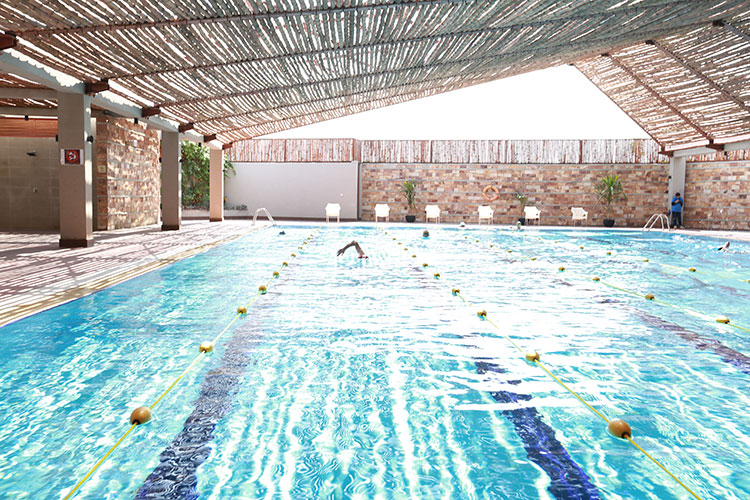
\includegraphics[width=\textwidth]{pool}
    \caption{An RGB image of a swimming pool.}
  \end{subfigure}
  \begin{subfigure}{.3\textwidth}
    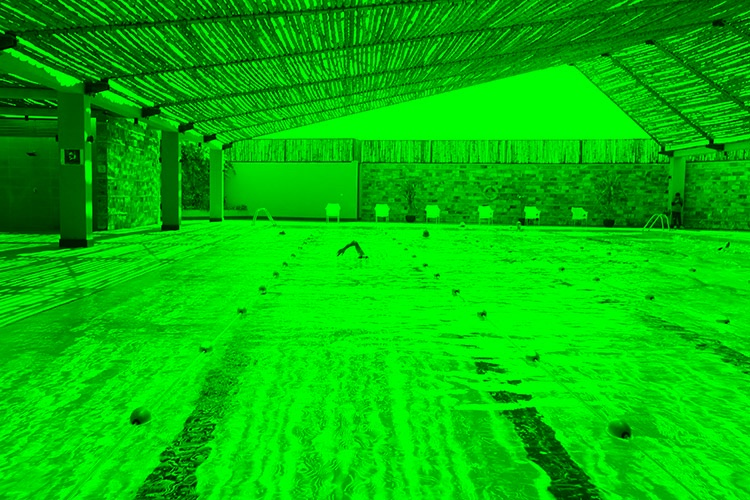
\includegraphics[width=\textwidth]{pool-sans-blue}
    \caption{The image with the blue channel turned off.}
  \end{subfigure}
  \begin{subfigure}{.3\textwidth}
    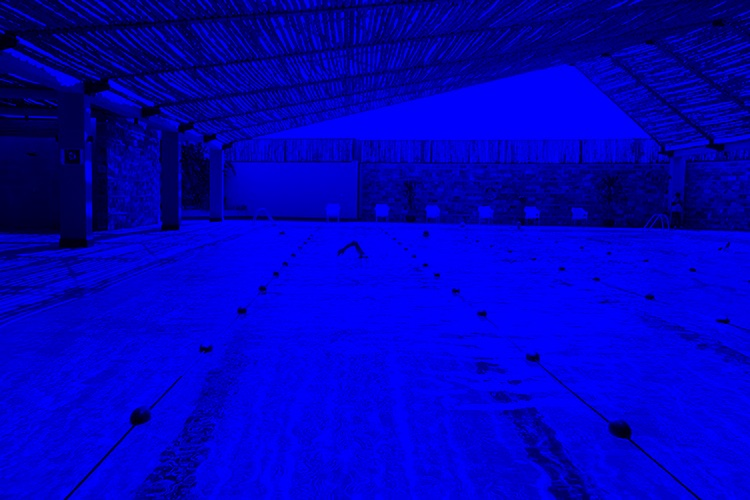
\includegraphics[width=\textwidth]{pool-only-blue}
    \caption{The original image with only the blue channel turned on.}
  \end{subfigure}
  \caption{Example of channel suppression.}
  \label{fig:channel}
\end{figure}

\subsection{Rotation}
Given a square image, i.e. one whose width is equal to its height, this operation generates a new image that contains rotations of the original image. Figure \ref{fig:rotate} shows an example of applying the operation. The resulting image has twice the dimensions of the original image, i.e. twice the width and twice the height.

\begin{figure}
  \centering
  \begin{subfigure}{.2\textwidth}
    
\includegraphics[scale=.5]{hu-logo}
    \caption{A square image.}
  \end{subfigure}
  \begin{subfigure}[c]{.35\textwidth}
    
\includegraphics[scale=.5]{hu-logo-rotated}
    \caption{The image obtained as a result of applying rotations to the original image.}
  \end{subfigure}
  \caption{Example of rotation.}
  \label{fig:rotate}
\end{figure}

\subsection{Applying a Mask}

A mask specifies certain \textit{weights} and applying the mask to an image entails replacing the value of each pixel in the image with a \textit{weighted sum} or \textit{weighted average} of the values of its \textit{neighbors}. The weights and the neighbors to consider for the average are specified by the mask.

The  mask is an $n \times n$ array of integers representing weights. For our purposes, $n$ must be odd. This means that the $n \times n$ array has a well defined center--the \textit{origin}. The weights in the mask can be arbitrary integers--positive, negative, or zero.

For each pixel in the input image, think of the mask as being placed on top of the image so its origin is on the pixel we wish to examine. The intensity value of each pixel under the mask is multiplied by the corresponding value in the mask that covers it. These products are added together. Always use the original values for each pixel for each mask calculation, not the new values you compute as you process the image.

For example, refer to Figure \ref{fig:mask-full}, which shows the  $3 \times 3$ mask,
\[
  \left[
    \begin{array}{ccc}
      1 & 3 & 1\\
      3 & 5 & 3\\
      1 & 3 & 1\\
    \end{array}          
  \right]
\]
and an image on which we want to perform the mask computation. Suppose we want to compute the result of the mask computation for pixel $e$. This result would be:
\[
  a + 3b + c + 3d + 5e + 3f + g + 3h + i
\]
Some masks require a \textit{weighted average} instead of a weighted sum. The weighted average in the case of Figure \ref{fig:mask-full} for pixel $e$ would be:
\[
  \frac{a + 3b + c + 3d + 5e + 3f + g + 3h + i} {1 + 3 + 1 + 3 + 5 + 3 + 1 + 3 + 1}
\]
Instead of doing this calculation for each channel individually, use the average value of the red, green, and blue channels. For example, if the pixel is given by $(r, g, b) = (107, 9, 218)$, then use $(107 + 9 + 218)//3 = 111$ for each channel. This effectively converts the image to grayscale.

Note that sometimes when you center the mask over a pixel you want to operate on, the mask will hang over the edge of the image. In this case, compute the weighted sum of only those pixels the mask covers. For the example shown in Figure \ref{fig:mask-hang}, the weighted sum for the pixel $e$ is given by:
\[
  3b + c + 5e + 3f + 3h + i
\]
and the weighted average is as follows. Integer division is used to ensure that pixel intensities are integers.
\[
  \frac{3b + c + 5e + 3f + 3h + i}{3+1+5+3+3+1}
\]

\begin{figure}
  \centering
  \begin{subfigure}{.48\textwidth}
    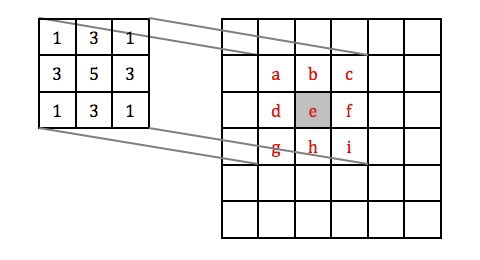
\includegraphics[width=\textwidth]{mask1}
    \caption{Overlay the $3 \times 3$ mask over the image so it is centered on pixel $e$ to compute the new value for pixel $e$.}\label{fig:mask-full}
  \end{subfigure}
  \begin{subfigure}[c]{.48\textwidth}
    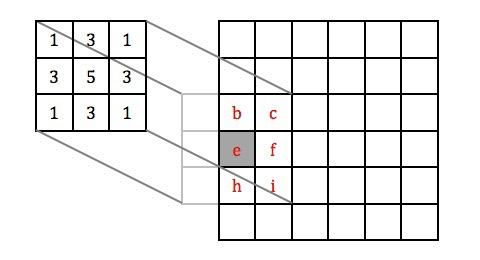
\includegraphics[width=\textwidth]{mask2}
    \caption{If the mask hangs over the edge of the image, use only those mask values that cover the image in the weighted sum.}\label{fig:mask-hang}
  \end{subfigure}
  \caption{Applying a mask to an image.}
  \label{fig:mask}
\end{figure}

\subsubsection{Applications of Masks}

Applying different masks leads to different properties. For example, applying the following mask above leads to blurring of the image. Figures \ref{fig:mask-orig} and \ref{fig:mask-blur} show the blurring effect of this mask. Note that color information is lost as mentioned above.
\[
  \left[
    \begin{array}{ccccc}
      2 & 4 & 5 & 4 & 2\\
      4 & 9 & 12 & 9 & 4\\
      5 & 12 & 15 & 12 & 5\\
      4 & 9 & 12 & 9 & 4\\
      2 & 4 & 5 & 4 & 2\\
    \end{array}          
  \right]
\]

Another application we use in an implementation of \textit{Canny Edge Detection} using \textit{Sobel Operators}. Once the image has been blurred as above, two more \textit{filters}, or masks, (the Sobel operators) are applied in succession to the blurred image. These filters determine the change in intensity, which approximates the horizontal and vertical derivatives.
\[
  G_x =   \left[
    \begin{array}{ccc}
      -1 & 0 & 1\\
      -2 & 0 & 2\\
      -1 & 0 & 1
    \end{array}
      \right], \quad
  G_y =   \left[
    \begin{array}{ccc}
      -1 & -2 & -1\\
      0 & 0 & 0\\
      1 & 2 & 1
    \end{array}    
  \right]
\]
. After these operations are applied one after the other to the blurred image, the values obtained are used to search for edges based on the magnitude and direction of the change in intensity. An example of the final result is shown in Figure \ref{fig:mask-edge}.

\begin{figure}
  \centering
  \begin{subfigure}{.31\textwidth}
    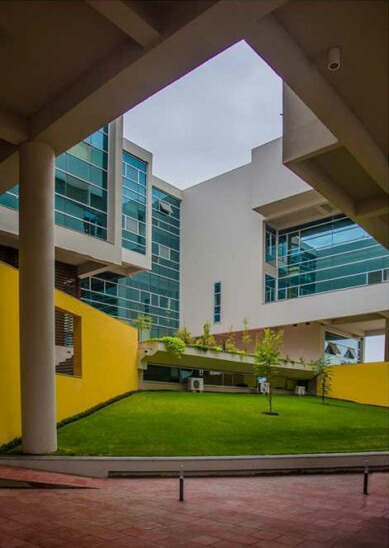
\includegraphics[width=\textwidth]{campus}
    \caption{An image with sharp details and several lines.}\label{fig:mask-orig}
  \end{subfigure}
  \begin{subfigure}[c]{.31\textwidth}
    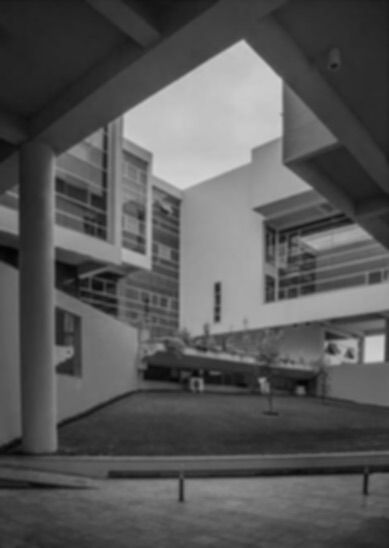
\includegraphics[width=\textwidth]{campus-blur}
    \caption{Result of applying the blur mask to the original image.}\label{fig:mask-blur}
  \end{subfigure}
  \begin{subfigure}[c]{.31\textwidth}
    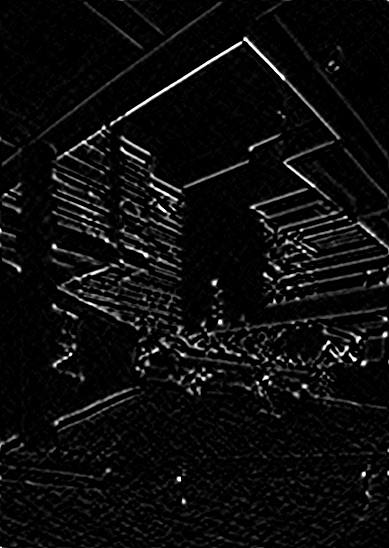
\includegraphics[width=\textwidth]{campus-edge-detect}
    \caption{Result of applying the Sobel filters to the blurred image.}\label{fig:mask-edge}
  \end{subfigure}
  \caption{Blurring and detection of edges in an image using masks.}
  \label{fig:mask-apply}
\end{figure}

\section{Image}

We treat an image as a grid of \textit{pixels} where each pixel has an RGB value indicating the red, green, and blue intensities of the pixel. An image has \textit{dimensions}, namely \textit{width} and \textit{height}, which determine the number of \textit{rows} and \textit{columns} in the image. Every pixel in the image is at a unique combination of row and column numbers which can therefore be used as coordinate system in the image. An image with width $w$ and height $h$ is said to be of size $w\times h$. Figure \ref{fig:img-dim} shows the column and row numbers in a $w\times h$ image along with the resulting pixel coordinates. Note that the coordinate is just a means to locate a pixel in the image, it is not the value stored at the pixel. The value stored at a pixel a triplet denoting the red, green, and blue intensities respectively.

We will work with a \textit{flattened} representation of an image. That is, we will store the pixel values in a 1-dimensional list structure as opposed to 2-dimensional structure. The list stores pixel values as they appear in the image from left to right and top to bottom. Figure \ref{fig:img-rgb} shows a $5\times 5$ image with some supposed RGB values. Note that each value would be a triplet of integers, each integer between 0 and 255 inclusive. Using our representation, the image in Figure \ref{fig:img-rgb} will be represented as the list:
\[
  [a, b, c, d, e, f, g, h, i, j, k, l, m, n, o, p, q, r, s, t, u, v, w, x, y]
\]

\begin{figure}
  \begin{subfigure}{.65\textwidth}
    \small
    \begin{tabular}{c*{6}{c|}}
      & \colheader{} & \multicolumn{5}{c}{Columns}\\
      \colheader{} &\colheader{} & \colheader{0} & \colheader{1} & \colheader{2} & \colheader{\ldots} & \colheader{$(w-1)$} \\\cline{3-7}
      \multirow{4}{*}{\rotatebox[origin=c]{90}{Rows}} &  0 & $(0, 0)$ & $(0, 1)$ & $(0, 2)$ & $\ldots$ & $(0, w-1)$ \\\cline{3-7}
      &  1 & $(1, 0)$ & $(1, 1)$ & $(1, 2)$ & $\ldots$ & $(1, w-1)$ \\\cline{3-7}
      &  2 & $(2, 0)$ & $(2, 1)$ & $(2, 2)$ & $\ldots$ & $(2, w-1)$ \\\cline{3-7}
      & \vdots & \vdots & \vdots & \vdots & $\ddots$ & \vdots \\\cline{3-7}
      &  $(h-1)$ & $(h-1, 0)$ & $(h-1, 1)$ & $(h-1, 2)$ & $\ldots$ & $(h-1, w-1)$ \\\cline{3-7}
    \end{tabular}
    \caption{Row and column numbers of an image with width $w$ and height $h$. Pixel coordinates are also shown.}\label{fig:img-dim}
  \end{subfigure}
  \begin{subfigure}{.3\textwidth}
    \[
      \begin{array}{|*{5}{c|}}
        \hline
        a & b & c & d & e\\\hline
        f & g & h & i & j\\\hline
        k & l & m & n & o\\\hline
        p & q & r & s & t\\\hline
        u & v & w & x & y\\\hline
      \end{array}      
    \]
    \caption{A $5\times 5$ image with supposed pixel values.}\label{fig:img-rgb}
  \end{subfigure}
  \caption{Image dimensions and pixel coordinates.}
  \label{fig:img}
\end{figure}

\section{Implementation Details and Tasks}

\subsection{Image Operations}

You have to implement the image operations shown in Listing \ref{lst:imgops} on Page \pageref{lst:imgops} and also included in the accompanying file \texttt{image\_operations.py}. These correspond to those illustrated in Section \ref{sec:imgops}. The operations manipulate an instance of our image type,  called \texttt{MyImage}. Note that none of the operations is destructive. That is, the original image is not modified. The result of an operation is returned as a new \texttt{MyImage} instance. 

\subsection{Image}

We implement our custom image type as \texttt{MyImage} as shown in Listing \ref{lst:img} on Page \pageref{lst:img} and also included in the accompanying file \texttt{myimage.py}. Note that the implementation uses \texttt{MyList} which is our implementation of the list. The given implementation is complete and you are not to change it except for the indicated line in \texttt{MyImage.\_\_init\_\_()}. You will change this line to use your implementation of \texttt{MyList}. This is the only change you are allowed to make in the implementation of \texttt{MyImage}.

\subsection{List}

We implement our custom list as \texttt{MyList} whose interface shown in Listing \ref{lst:lst} on Page \pageref{lst:lst} and also included in the accompanying file \texttt{mylist.py}. Note that the implementation is mostly complete except for the segments marked as \texttt{pass}. The implementation includes a mechanism to allow iteration over the list and using some other native python syntax with it.

You have to copy the implementation to \texttt{ArrayList} and \textsf{PointerList} which will implement the list using \href{https://www.programiz.com/python-programming/array}{python arrays} and pointers respectively. See the implementation of BST in Listing \ref{lst:bst} on Page \pageref{lst:bst} and also included in the accompanying file \texttt{bst.py} to understand pointers in python. You then have to modify the required line in \texttt{myimage}.py to use your type.

\section{Timing}

We want to perform a timing analysis on the execution of the image operations using our list implementations. Those details are forthcoming.

\section{Bonus}

You can earn bonus marks for implementing interesting image manipulation algorithms of your own. Please see the rubric for more details. Interesting submissions will be featured on the course's forthcoming web page.

\section{Credits}

This homework is adapted from Homework 3 of the Fall 2014 offering of 15-122: Principles of Imperative Computation at Carnegie Mellon University (CMU). Credit is due to \href{https://www.facebook.com/abdullah.zafar.547389}{Abdullah Zafar} for identifying it.

\newpage
\appendix
\section{Image Operations}
\lstinputlisting[language=python, frame=single, caption=Image Operations, label={lst:imgops}]{src/image_operations.py}

\newpage
\section{\texttt{MyImage}}
\lstinputlisting[language=python, frame=single, caption=Image Type, label={lst:img}]{src/myimage.py}

\newpage
\section{\texttt{MyList}}
\lstinputlisting[language=python, frame=single, caption=List Type, label={lst:lst}]{src/mylist.py}

\newpage
\section{Pointers in python}
\lstinputlisting[language=python, frame=single, caption=BST in python, label={lst:bst}]{src/bst.py}



% ''' Python debugging: https://realpython.com/python-debugging-pdb/
% '''

\end{document}
%%% Local Variables:
%%% mode: latex
%%% TeX-master: t
%%% End:
